\section{Experimental Evaluation}
\label{sec:evaluation}

In this section, we experimentally evaluate \dtn and compare it with other DTN software.

\subsection{Emulation Environment}
To evaluate \dtn in a realistic manner, we emulated up to 64 nodes in the network emulation framework \emph{Common Open Research Emulator} (CORE)~\cite{ahrenholz2010comparison}.
CORE can emulate nodes using Linux namespaces to allow the execution of native binary programs, which is not possible with purely simulation-based approaches like NS-3~\cite{riley2010ns,schwerdel2011tomato}.
All experiments were performed on Intel Xeon E5-2698 CPUs with 80 cores at 2.20 GHz and 256 GB RAM.
To execute the total number of 1,440 experiment runs, we used MACI, a framework for extensive and reproducible experiments~\cite{froemmgen2018maci}.

\subsubsection{DTN Software.}
We compared \dtn with three popular DTN software solutions.
\textit{Serval}\footurl{https://github.com/servalproject/serval-dna/tree/batphone-release-0.93} is a software suite centered around protocols designed for infra\-structure independent communication~\cite{gardner2011serval}.
To be able to transfer files in intermittently connected networks, Serval relies on Rhizome, a custom DTN bundle protocol with epidemic routing.
In our evaluation, we used the latest stable Serval release, which is from April 2016, since the recent development version has stability issues.
\textit{IBR-DTN}\footurl{https://github.com/ibrdtn/ibrdtn} is an implementation of BP Version 6, aimed to be lightweight and fast~\cite{doering2008ibr}.
For comparability, we use the epidemic routing extension instead of the default PRoPHET protocol used by IBR-DTN.
We use the current HEAD of the git repository to include the latest bug fixes.
\textit{Forban}\footurl{https://github.com/adulau/Forban} is mainly used as a local peer-to-peer file sharing application using an epidemic routing protocol based on HTTP.
We used the latest HEAD of the git repository, but had to introduce our own patches to make Forban usable.
%For \dtn, we use the at the moment of writing recent version 0.1.

% Similar to \dtn, these implementations 
% have their own neighbor discovery, depending on periodical announcements of the node status.
% For comparability reasons, we set the announcement interval to two seconds for all tests, since this is the sweet spot between resource usage and over-utilization of the network~\cite{baumgartner2017speak}.

\subsubsection{Payload Sizes.}
DTN software is used in multiple applications and scenarios.
Serval, e.g., offers the SMS-like application MeshMS for short text messages.
IBR-DTN can be used in environmental monitoring, where transmission of short audio recordings or images might be required. 
Therefore, we selected four different file sizes, representing a wide range of possible applications.
All files were generated randomly with the same seed for reproducibility in six sizes:

\begin{itemize}
    \item 
\textit{64 KiB} for compressed images or map data;
\item
\textit{1 MiB} representing small images or short audio recordings;
\item
\textit{5 MiB}, e.g., smartphone images and audio recordings;
\item
\textit{25 MiB} representing longer audio recordings or short videos;
\item
\textit{50 MiB} for HD videos typically recorded by smartphones;
\item
\textit{100 MiB}, e.g., 4k smartphone videos \cite{trono2015dtn,schildt2011ibr,baumgaertner2016serval}.
\end{itemize}


\subsubsection{Network Topologies.}
%We worked with two kinds of topology.
%First, 
We used a chain topology of three different lengths, where nodes are connected pairwise, to benchmark the different DTN software systems.
The first node is sending a bundle destinated to the last node in the chain.
To get the baseline performance of the interacting components, a chain of two nodes was used.
We measured the time it takes to read the data, serialize the bundle, send it over the network, deserialize it at the receiver and deliver it to the application.
With 32 nodes, the forwarding capabilities were investigated.
For an even larger scenario, we used 64 nodes, to evaluate how the DTN software systems behave when node numbers increase.
We used a bandwidth of 54 MBit/s to match the speed of an IEEE 802.11g network. 
%used in the mobile scenarios.

% Second, we used a \textbf{mobile} scenario with \textbf{64} randomly moving nodes.
% Each node was modelled to imitate human behavior in an area of 1.7 km$^2$ at a speed between 0.8 m/s and 1.9 m/s or rest for up to 60 seconds.
% We used 1, 8 and 16 sending nodes in different tests, where each sent a file either directed to a specific node or in case of Serval and Forban a broadcast bundle was used, since they are not able to send bundles directly.
% With this experiment, we can analyze how fast bundles are spread over the network under the same conditions for every software.
% IEEE 802.11g networks are still widely used, especially over long-range connections.
% Thus, we limited the bandwidth to 54 MBit/s and used a basic range model for the Wi-Fi nodes with 40 meters of range.

\subsubsection{Measurements.}
To measure CPU utilization for each process on every node, we used \textit{pidstat}, which is part of the \textit{sysstat} package\footnote{http://sebastien.godard.pagesperso-orange.fr/man\_pidstat.html}.
Additionally, \textit{bwm-ng}\footnote{https://github.com/vgropp/bwm-ng} was used for network statistics per node and network interface.
Finally, every used DTN software logged both the timestamp of sending and receiving bundles, such that a detailed analysis of transmission time and network distribution can be performed.


\subsection{Results}

\subsubsection{Transmission Times.}
\label{subsub:transmission_time}

\begin{figure}[t]
    \centering
  %  \begin{subfigure}[t]{0.5\columnwidth}
  %    \centering
        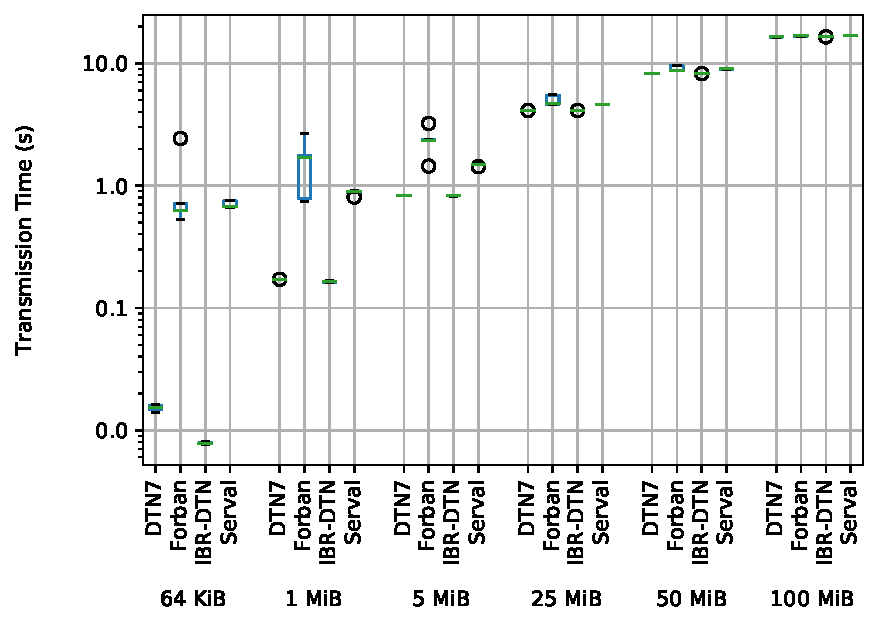
\includegraphics[width=0.8\columnwidth]{figs/chain-runtimes-2.pdf}
        \caption{Bundle transmission time for the 1-hop topology and different payload sizes}
        \label{fig:transmissions1}
  %    \end{subfigure}~
\end{figure}
\begin{figure}[h]
 %   \begin{subfigure}[t]{0.5\columnwidth}
        \centering
        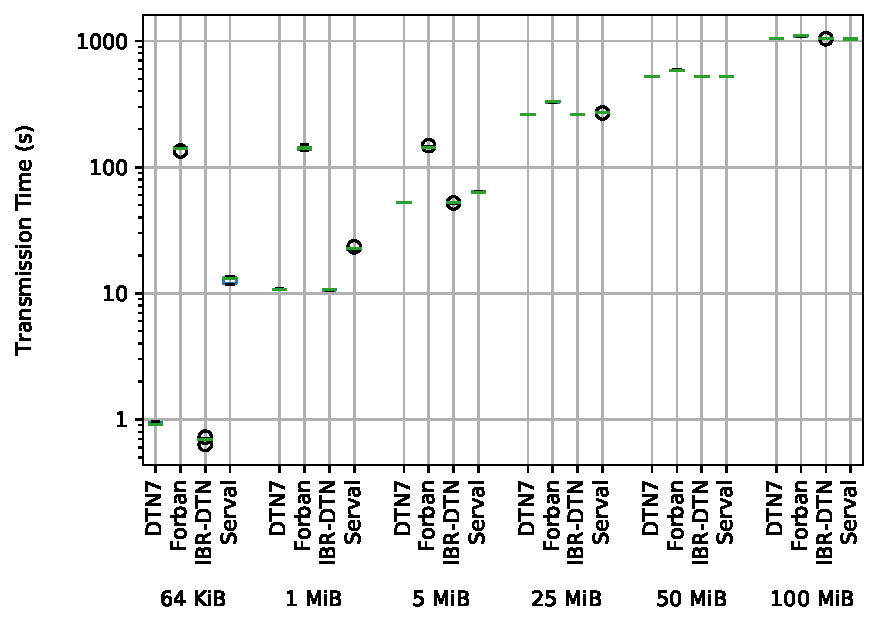
\includegraphics[width=0.8\columnwidth]{figs/chain-runtimes-64.pdf}
  %      \caption{64 hops}
 %   \end{subfigure}
    \caption{Bundle transmission time for the 64-hops topology and different payload sizes.}
    \label{fig:transmissions64}
\end{figure}

Figs.~\ref{fig:transmissions1} and \ref{fig:transmissions64} show the bundle transmission times on the y-axes and payload sizes on the x-axes for the 1-hop and 64-hops topologies, respectively.
Regardless of chain length and file size, \dtn and IBR-DTN are always the fastest DTN software systems.
The larger the files become, the transfer times of all DTN systems converge.
This is due to the network configuration.
All DTN systems manage to completely fill the 54 Mbit/s available, which is easier to achieve with larger files.
As a result, the transfer times for large files hardly vary at all.

For a single hop, Forban and Serval take about the same time for transmitting files (e.g., about 0.6 seconds for 64 KiB files), but Forban shows a higher variance.
For longer chains and files below 50 MiB, the differences between Forban and Serval are more noticable.
\dtn, however, is still up to 140 times (64 KiB over 1 hop) faster than Serval. %\dtn converges when approaching 100 MiB files.
Particularly in chat or text based applications, the speed advantage of \dtn can be crucial if a message arrives below 0.01 seconds rather than after one second.

These results indicate that both BP6 and BP7 have a relatively small protocol overhead compared to the protocols used by Serval and Forban, which is especially noticeable for small files.
The larger the files or the longer the chain, the less weight the low protocol overhead carries.
Furthermore, it is also remarkable that \dtn, which is written in Go, does not take longer to transmit larger files from end to end in the chain, although IBR-DTN is implemented in C++ and optimized for speed.
In terms of transmission speeds, Forban takes longer than the other DTN software systems, although differences get smaller the bigger the files are. One explanation is that Forban has a pull-based approach where it actively downloads new bundles after an announcement was received. Therefore, the announcement interval is a natural barrier. If quick data exchange is necessary, the other solutions provide better performance.

\begin{figure}[t]
%    \centering
\hspace{-15mm}
    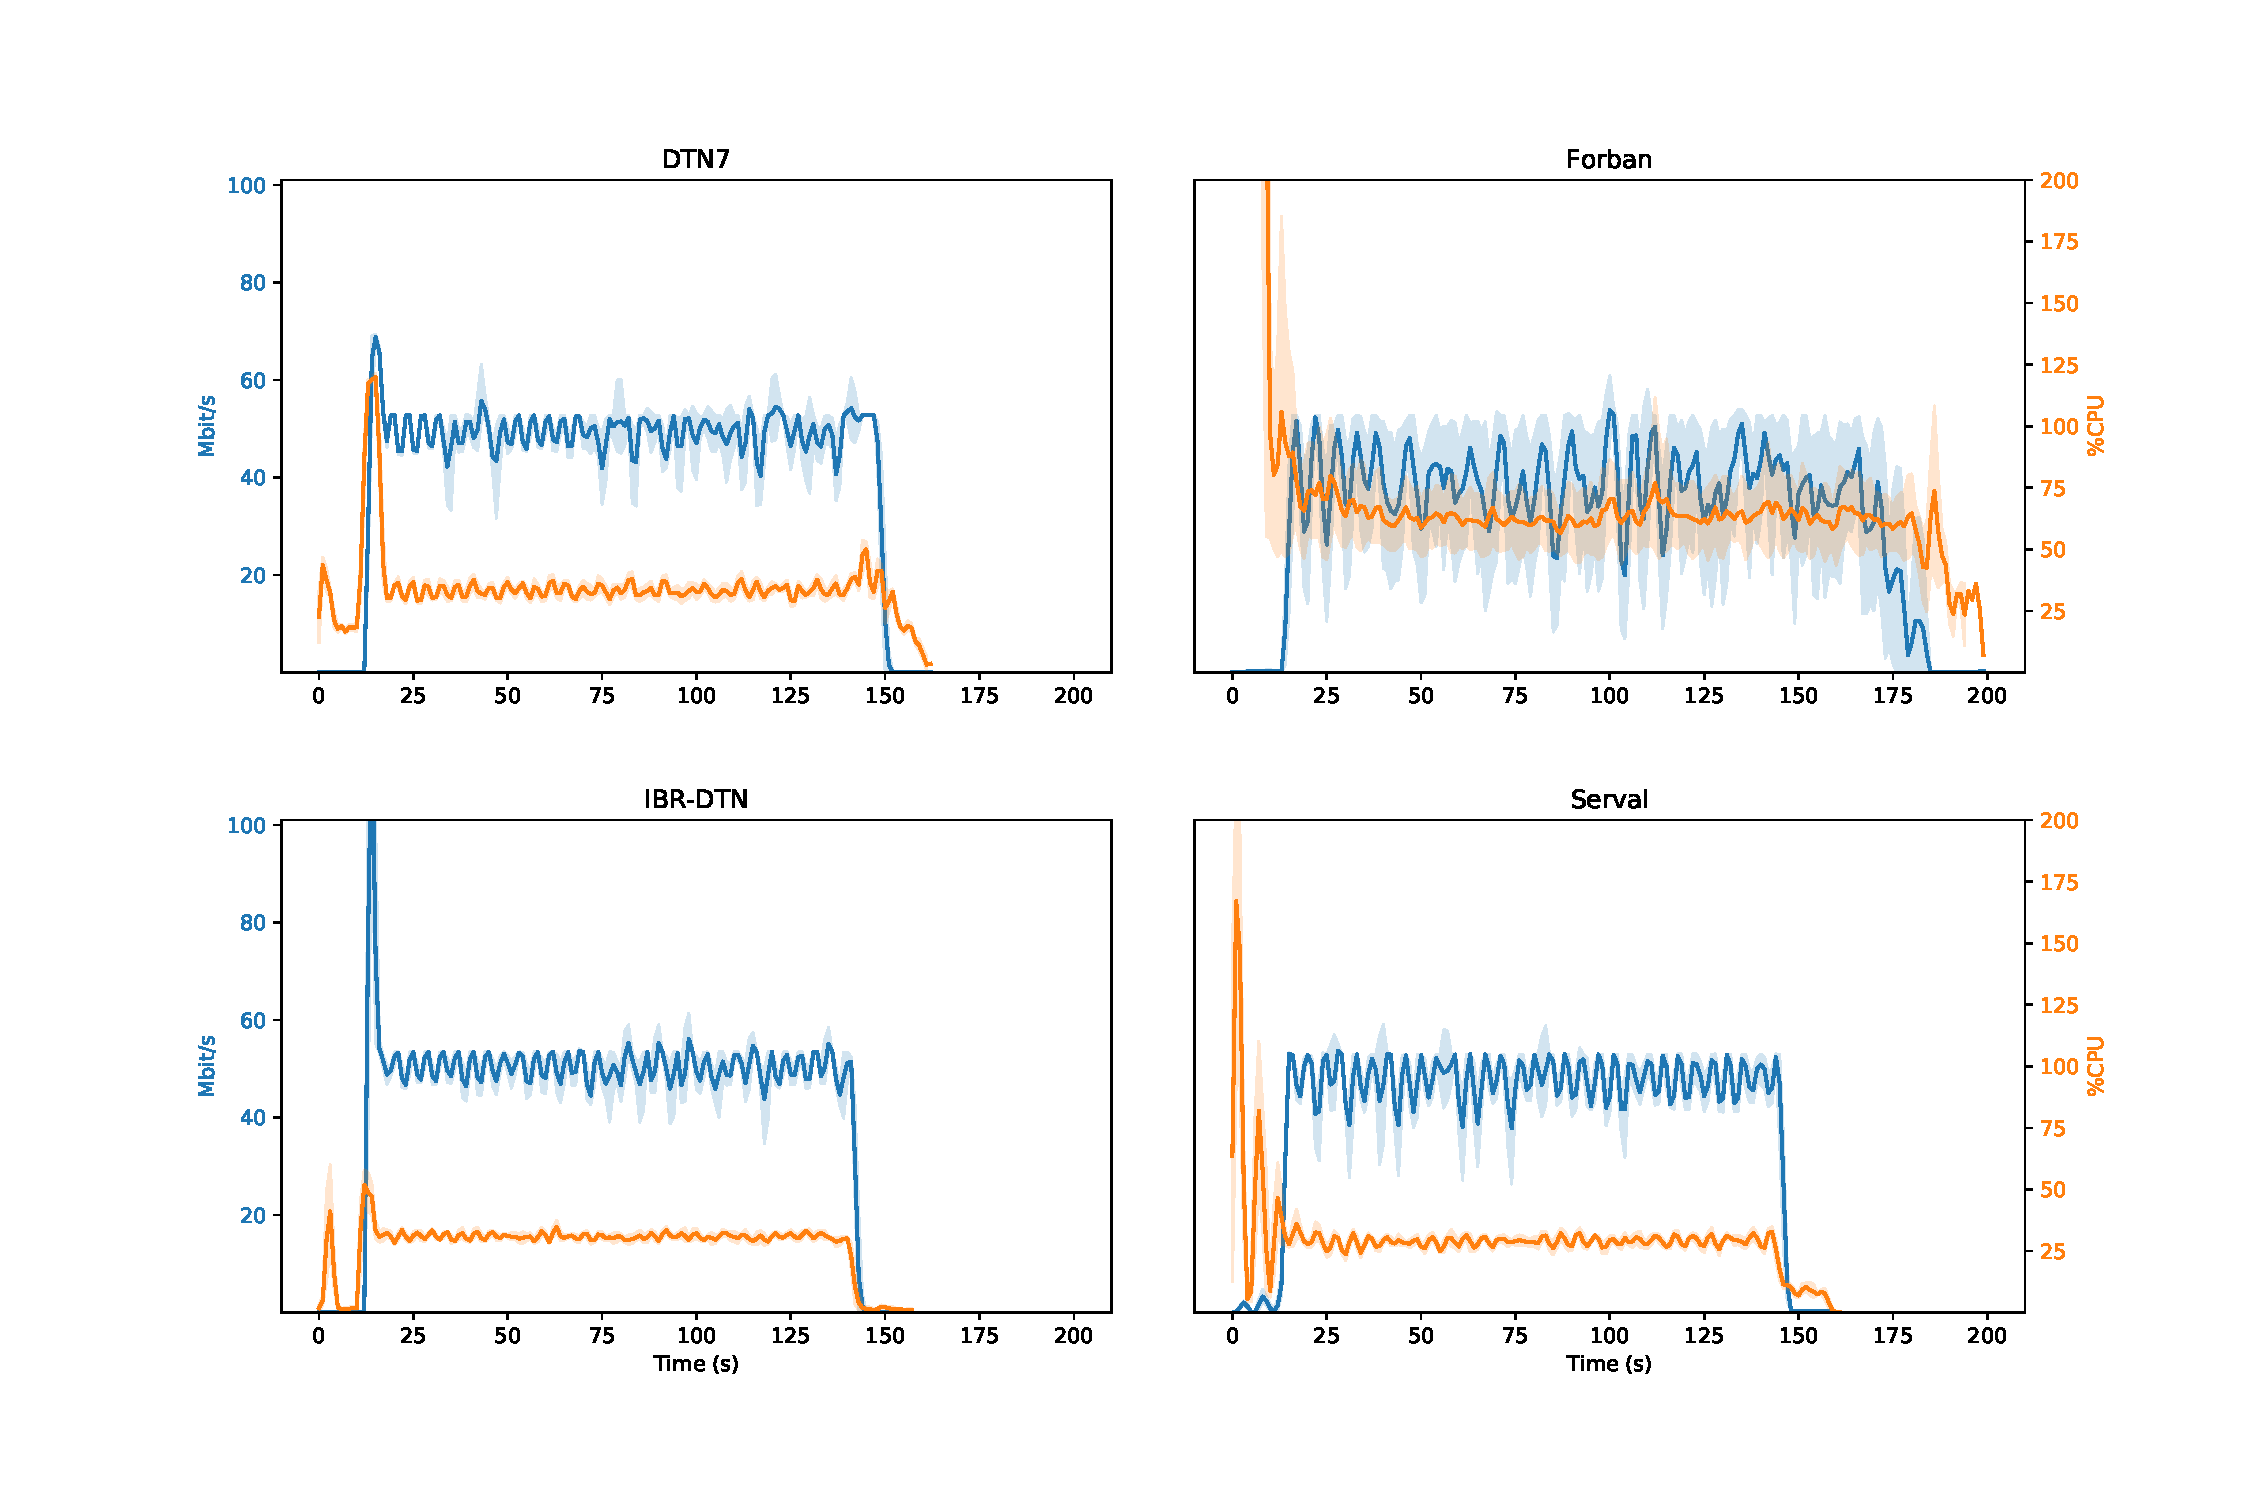
\includegraphics[width=1.2\columnwidth]{figs/cpu_network.pdf}
    \caption{CPU and network usage for transmitting 25 MiB over 32 hops.}
    \label{fig:cpu_net}
\end{figure}


\subsubsection{CPU Usage and Network Utilization.}


Fig.~\ref{fig:cpu_net} shows CPU usage and network utilization for transmitting 25 MiB over 32 hops.
On the x-axes, the time for the entire experiment in seconds is shown, the left y-axes denote the network usage in Mbit/s and the right y-axes show the CPU usage in \%, both of the entire network.
The bold graphs denote the sum over all nodes, averaged over all experiment repetitions.
The shaded areas denote the error band.

\dtn requires about 34.3\% of the available CPU (standard deviation of 16.7\%).
At the beginning of an experiment, \dtn shows a short peak in CPU usage resulting from the first node, where the file is converted to base64, sent to the \dtn AA, which decodes the file again, packs it into a bundle, and starts the transmission.
Further nodes only have to retransmit the bundle and do not require the steps mentioned above.
Forban uses about 163.1\% CPU (646.3\%).
Forban shows a small peak at the start of the experiment, indicating the overhead when starting its daemons, where four Python interpreters have to be started.
Additionally, the file has to be hashed at the beginning of the experiment.
Serval consumes 29.3\% (24.6\%) CPU.
Serval has an additional hashing step, which results in higher CPU load at the start of the experiment.
With only 26.9\% (13.1\%), IBR-DTN is the most efficient tested DTN software in terms of CPU usage.



In terms of network usage, \dtn reaches about 42.0 Mbit/s (19.7 Mbit/s) for transmitting bundles from node to node, while Forban achieves about 32.8 Mbit/s (22.8 Mbit/s).
IBR-DTN and Serval achieve 42.3 Mbit/s (23.7 Mbit/s) and 39.5 Mbit/s (20.0 Mbit/s), respectively.
Although the theoretical total network load for the entire network can be up to 1.674 Gbit/s, the tested DTN software systems used only the maximum bandwidth per link, which is 54 Mbit/s, in peak situations.
This indicates that every DTN software needs to receive the entire bundle before transmitting it to the next node.


To summarize, \dtn requires slightly more CPU utilization than IBR-DTN and Serval, but has the advantage of transmitting files faster than all other DTN systems in most cases, as shown in Section~\ref{subsub:transmission_time}.

% \subsection{Mobile Scenario}


% To evaluate the practical usage of \dtn, we conducted a series of experiments using a mesh topology in the mobile scenario.
% We evaluated when and how many bundles arrived at the destination.


% Table~\ref{tab:arrivals} shows that \dtn needs the longest time to deliver a file in the mobile scenario, reaching around 614 seconds for a 25 MiB file.
% %the difference is most significant for 25 MiB files.
% The other DTN software systems require all below 300 seconds, regardless of the file size.
% In experiments with eight senders, the results are similar, as shown in Fig. TODO.

% The \dtn results are due to the used CL, namely MTCP in our proof-of-concept version.
% Since there is no mechanism to detect a connection loss with MTCP, the underlying TCP socket retries to send a packet using an exponential backoff waiting time.
% Only if the last retry fails, the application (in this case \dtn) is notified and can handle the issue appropriately.
% Using a more sophisticated CL like TCPCL, this issue can be fixed in future \dtn releases.

% \begin{table}[t]
% \centering
% \caption{Mean arrival times in seconds from sender to receiver, with one sender.} 
% \vspace{5mm}
% \begin{tabular}{l|llll}
% \hline
% Software/Size & 64 KiB & 1 MiB  & 5 MiB  & 25 MiB \\ \hline
% \dtn          & 306.71 & 309.14 & 328.82 & 614.92 \\
% Forban        & 245.48 & 279.81 & 281.67 & 290.66 \\
% IBR-DTN       & 276.65 & 278.22 & 279.23 & 281.88 \\
% Serval        & 205.18 & 286.34 & 286.41 & 290.38 \\ \hline
% \end{tabular}
% \label{tab:arrivals}
% \end{table}

% Using one sender, the file reached the destination in all experiments and all DTN software systems.
% Using eight senders, all files reached the destination in most experiments.
% IBR-DTN and \dtn achieved an average of 7.7 out of 8  with 64 KiB files. With 25 MiB using \dtn, an average of 4.3 out of 8 files arrived at the destination.
% This is consistent with the results achieved in other experiments with 25 MiB files.

% %To summarize, \dtn is a BP7 implementation that achieves results as good as other DTN softwares, in many cases even better.
% %With further optimizations and ongoing development, \dtn will be a great baseline implementation for upcomming research and development in the filed of DTN.